%%%%%%%%%%%%%%%%%%%%%%%%%%%%%%%%%%%%%%%%%%%%%%%%%%%%%%%%%%%%%%%%%%%%%
% APPENDIXES
%%%%%%%%%%%%%%%%%%%%%%%%%%%%%%%%%%%%%%%%%%%%%%%%%%%%%%%%%%%%%%%%%%%%%
%
% Use \appendix if there is only one appendix.
\appendix
The mapping of the physics tendencies from the physics grid to the GLL grid is done with tensor-cubic Lagrange interpolation. The elements of the cubed-sphere in SE are created from an equi-angular gnomonic projection. Consider one element $(\alpha,\beta) \in \left[ \alpha^{(elem)}_1,\alpha^{(elem)}_2 \right]\times \left[ \beta^{(elem)}_1,\beta^{(elem)}_2\right]$, where $(\alpha,\beta)$ are central angle coordinates and $\alpha^{(elem)}_1$ and $\alpha^{(elem)}_2$ are the minimum and maximum central angles in the $\alpha$-coordinate direction, respectively, and similarly for $\beta$. Let $\Delta \alpha^{(elem)}=\alpha^{(elem)}_2-\alpha^{(elem)}_1$ and $\Delta \beta^{(elem)}=\beta^{(elem)}_2-\beta^{(elem)}_1$. The physics grid cell central angle centers are located at
\begin{multline}
(\alpha^{(pg)}_i,\beta^{(pg)}_j)= \Big[ \alpha^{(elem)}_1+\left(i-\tfrac{1}{2}\right) \Delta \alpha^{(pg)},\\
                                      \beta^{(elem)}_1+\left(j-\tfrac{1}{2}\right) \Delta \beta^{(pg)}\Big],
\end{multline}
where $\Delta \alpha^{(pg)}=\Delta \beta^{(pg)}=\frac{\Delta \alpha^{(elem)}}{pg}=\frac{\Delta \beta^{(elem)}}{pg}$. The interpolation is performed in central-angle coordinates using tensor product cubic interpolation. For elements located on a cubed-sphere edge or corner the coordinate system for neighboring elements may be on a different panel. To take into account this coordinate change the central angle locations of physics grid cell centers located on other panels are transformed to the coordinate system of the panel the element in question is located on \cite[the transformations are given in, e.g.,  ][]{NTL2005MWRb}. An illustration is given in Figure \ref{fig:mapping} for an element located in the lower left corner of a panel. The element in question is $(\xi,\chi)\in (-1,1)^2$ where, for simplicity, we have transformed the element coordinates into normalized coordinates $(\xi,\chi) = \left( \frac{ 2\left(\alpha^{(pg)}-\alpha^{(elem)}_1\right)}{\Delta \alpha^{(elem)}}-1,\frac{2\left( \beta^{(pg)}-\beta^{(elem)}_1\right)}{\Delta \beta^{(elem)}}-1\right)$; also used internally in the SE dynamical core \citep[see, e.g., section 3.3 in ][]{LetAl2018JAMES}. The GLL points are located at -1,$-1/\sqrt{1}$, $1/\sqrt{5}$, and 1 in each coordinate direction. Near the edges/corners of an element cubic extrapolation is used if the centered stencil expands beyond the panel.

\begin{figure}[t]
\begin{center}
\noindent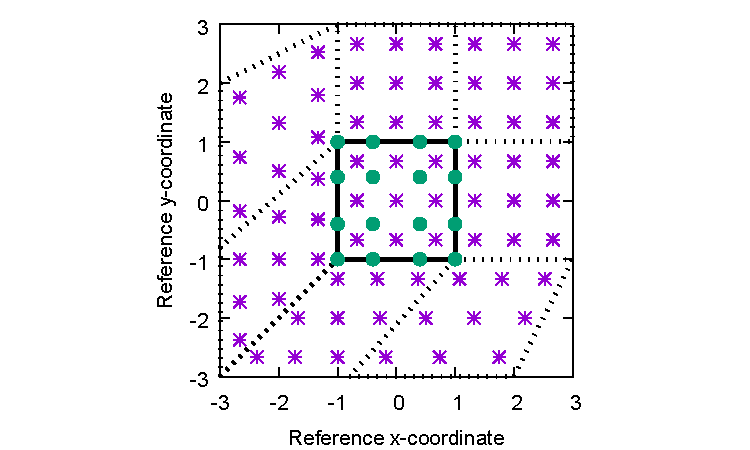
\includegraphics[width=20pc,angle=0]{chapter4/mapping.pdf}\\
\end{center}
\caption{Schematic of the coordinate system in which the dimensionally split cubic Lagrange interpolation is computed.  The physics grid centers are marked with asterisks and the GLL points, we are interpolating to, with solid filled circles. The element in which the GLL points are located is  bounded by  thick black lines and located in the lower left corner of a panel. The stippled lines mark the boundaries of the remaining elements. For simplicity we are using the normalized coordinate centered at the element on which the GLL points we are interpolating to are located. Note that the coordinates for points on neighboring panels (using a different local coordinate system) must be transformed to the coordinate system of the element in question.}
\label{fig:mapping}
\end{figure}

\subsection{Defining $\Delta t_{phys}$ across resolutions}\label{sec:app1}
 \cite{HR2018JAMES} developed a moist bubble test, which indicate that time-truncation errors are large at high resolution (about $50km$ or less) using more conventional values for the physics time-step. The test may be able to provide insight on a reasonable scaling of $\Delta t_{phys}$ across resolutions in more complex configurations. In the test a set of non-rotating simulations are initialized with a warm, super-saturated moist bubble, and the grid spacing and bubble radius are simultaneously reduced by the same factor in each run through varying the planetary radius. The test was designed to mimic the reduction in buoyancy length scales that occur when the model resolution is increased in more complex configurations \citep{HETAL2006JCLIM,HR2018JAMES}. 
 
The moist bubble test is performed with CAM-SE-CSLAM and coupled to the simple condensation routine of \cite{K1969MM} across five different resolutions (pertaining to the $ne30$, $ne40$, $ne60$, $ne80$, and $ne120$ grids). The results are expressed as the minimum $\omega$ throughout each one day simulation, and shown in Figure~\ref{fig:bubble}. Two sets of simulations are performed with both $pg3$ and $pg2$, one with $\Delta t_{phys}$ determined by equation~\eqref{eq:dt-scale}, and an equivalent set of simulations with $\Delta t_{phys} = 1800s$ for all resolutions. 

\begin{figure}[t]
\begin{center}
\noindent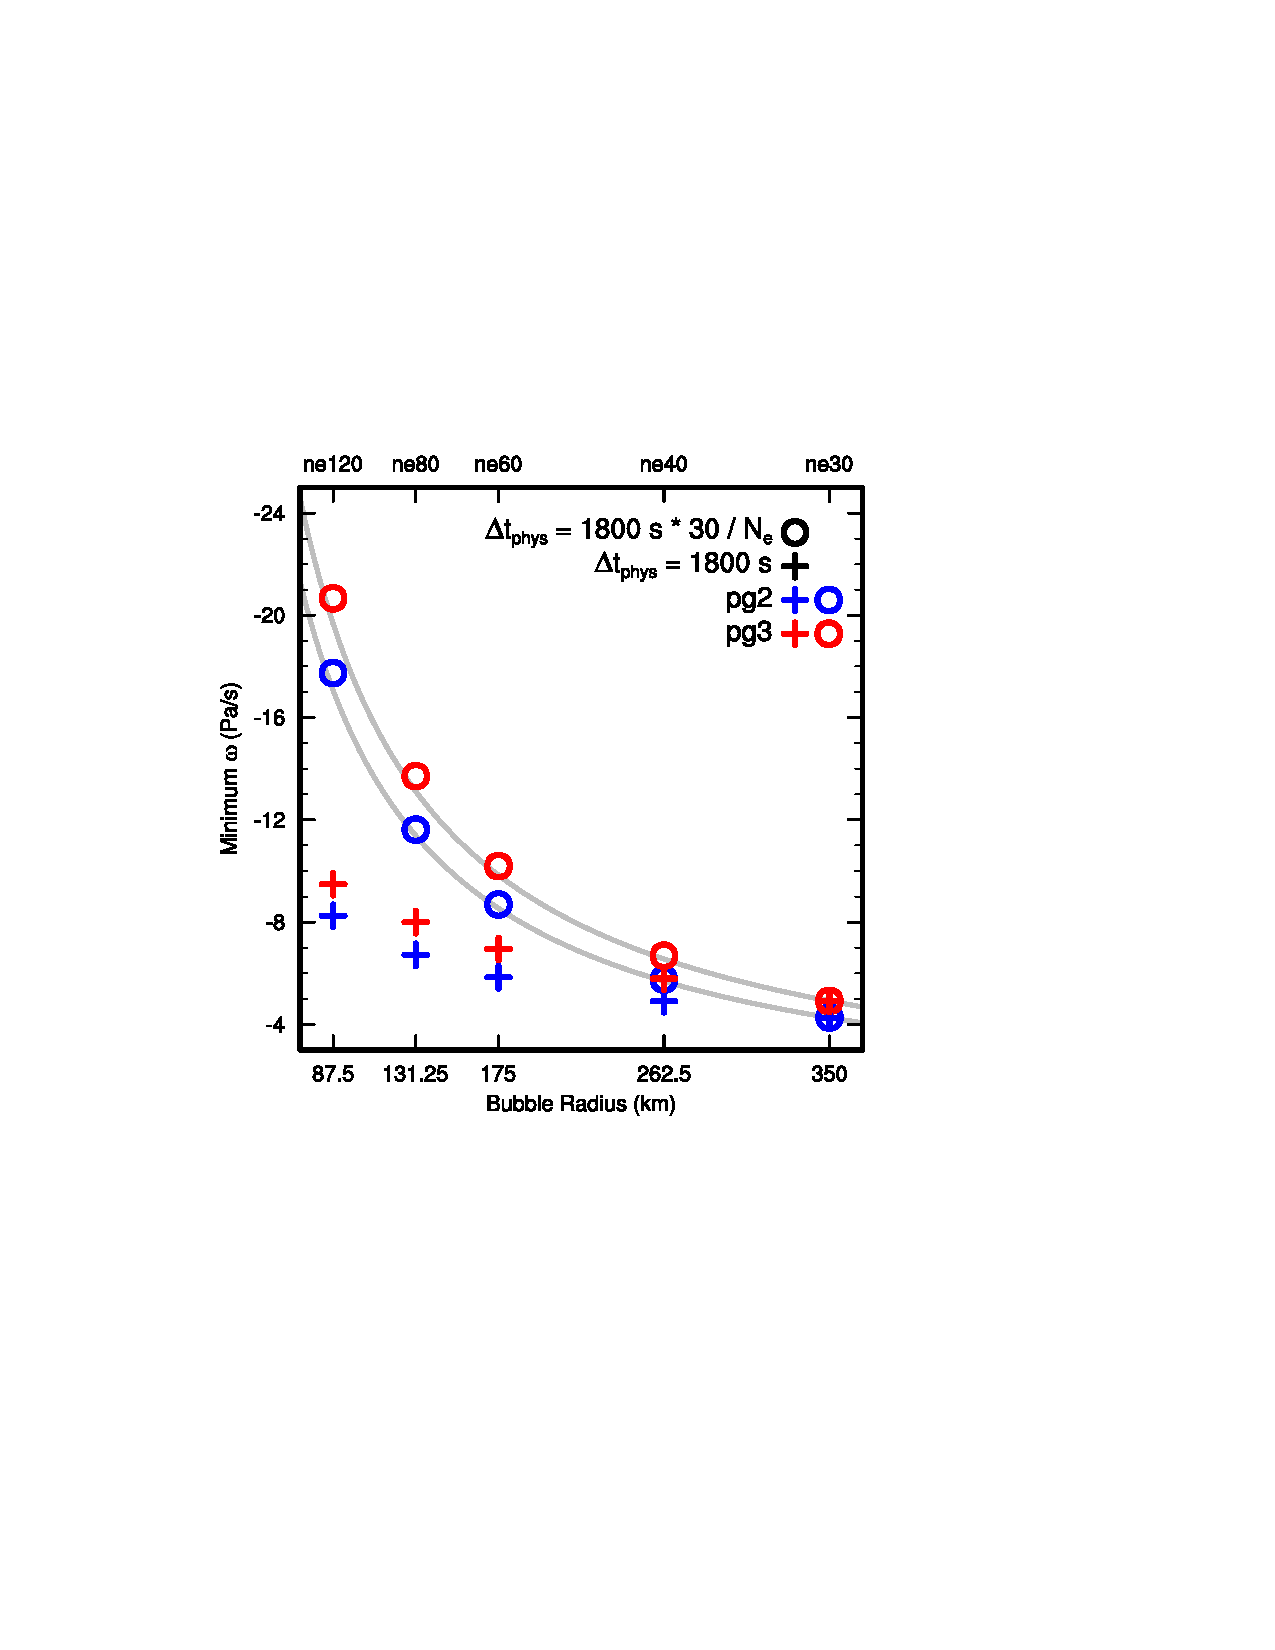
\includegraphics[width=20pc,angle=0]{chapter5/bubble_test.pdf}\\
\end{center}
\caption{The magnitude of $\omega$ in the $pg3$ solutions are systematically larger than the $pg2$ solutions, which is primarily a result of the damping effect of integrating the basis functions over a larger control volume.}
\label{fig:bubble}
\end{figure}

With the diameters of the bubbles set proportional to $\Delta x_{dyn}$, \cite{HR2018JAMES} has shown that $\omega$ converges to the scaling of equation~\eqref{eq:w-scale} in the limit of small $\Delta t_{phys}$, where small $\Delta t_{phys}$ refers to the CFL limiting time-step used by the dynamics. Equation~\eqref{eq:w-scale} is overlain as grey lines in Figure~\ref{fig:bubble}, with $ne30$ being the reference resolution. The solutions using $\Delta t_{phys}$ from equation~\eqref{eq:dt-scale} follow the scaling, whereas fixing $\Delta t_{phys} = 1800s$ across resolutions damps the solution relative to the analytical solution, progressively more so at higher resolutions. If $\Delta t_{phys}$ is too large, the solution has non-negligible error, which is avoided through scaling $\Delta t_{phys}$ according to equation~\eqref{eq:dt-scale}.

To get a a handle on whether the test is useful for understanding more realistic configurations, four aqua-planet simulations are performed using the CAM6 physics package. A pair of $ne30pg2$ simulations, one in which $\Delta t_{phys}$ is set to the appropriate value from equation~\eqref{eq:dt-scale} ($1800s$), and another where it is set to the $\Delta t_{phys}$ corresponding to the $ne20$ resolution ($2700s$). Similarly, a pair of $ne120pg2$ simulations are performed, one with $\Delta t_{phys}$ set to the value from equation~\eqref{eq:dt-scale} ($450s$), and one with $\Delta t_{phys}$ set to the $ne80$ value ($675s$). 

\begin{figure}[t]
\begin{center}
\noindent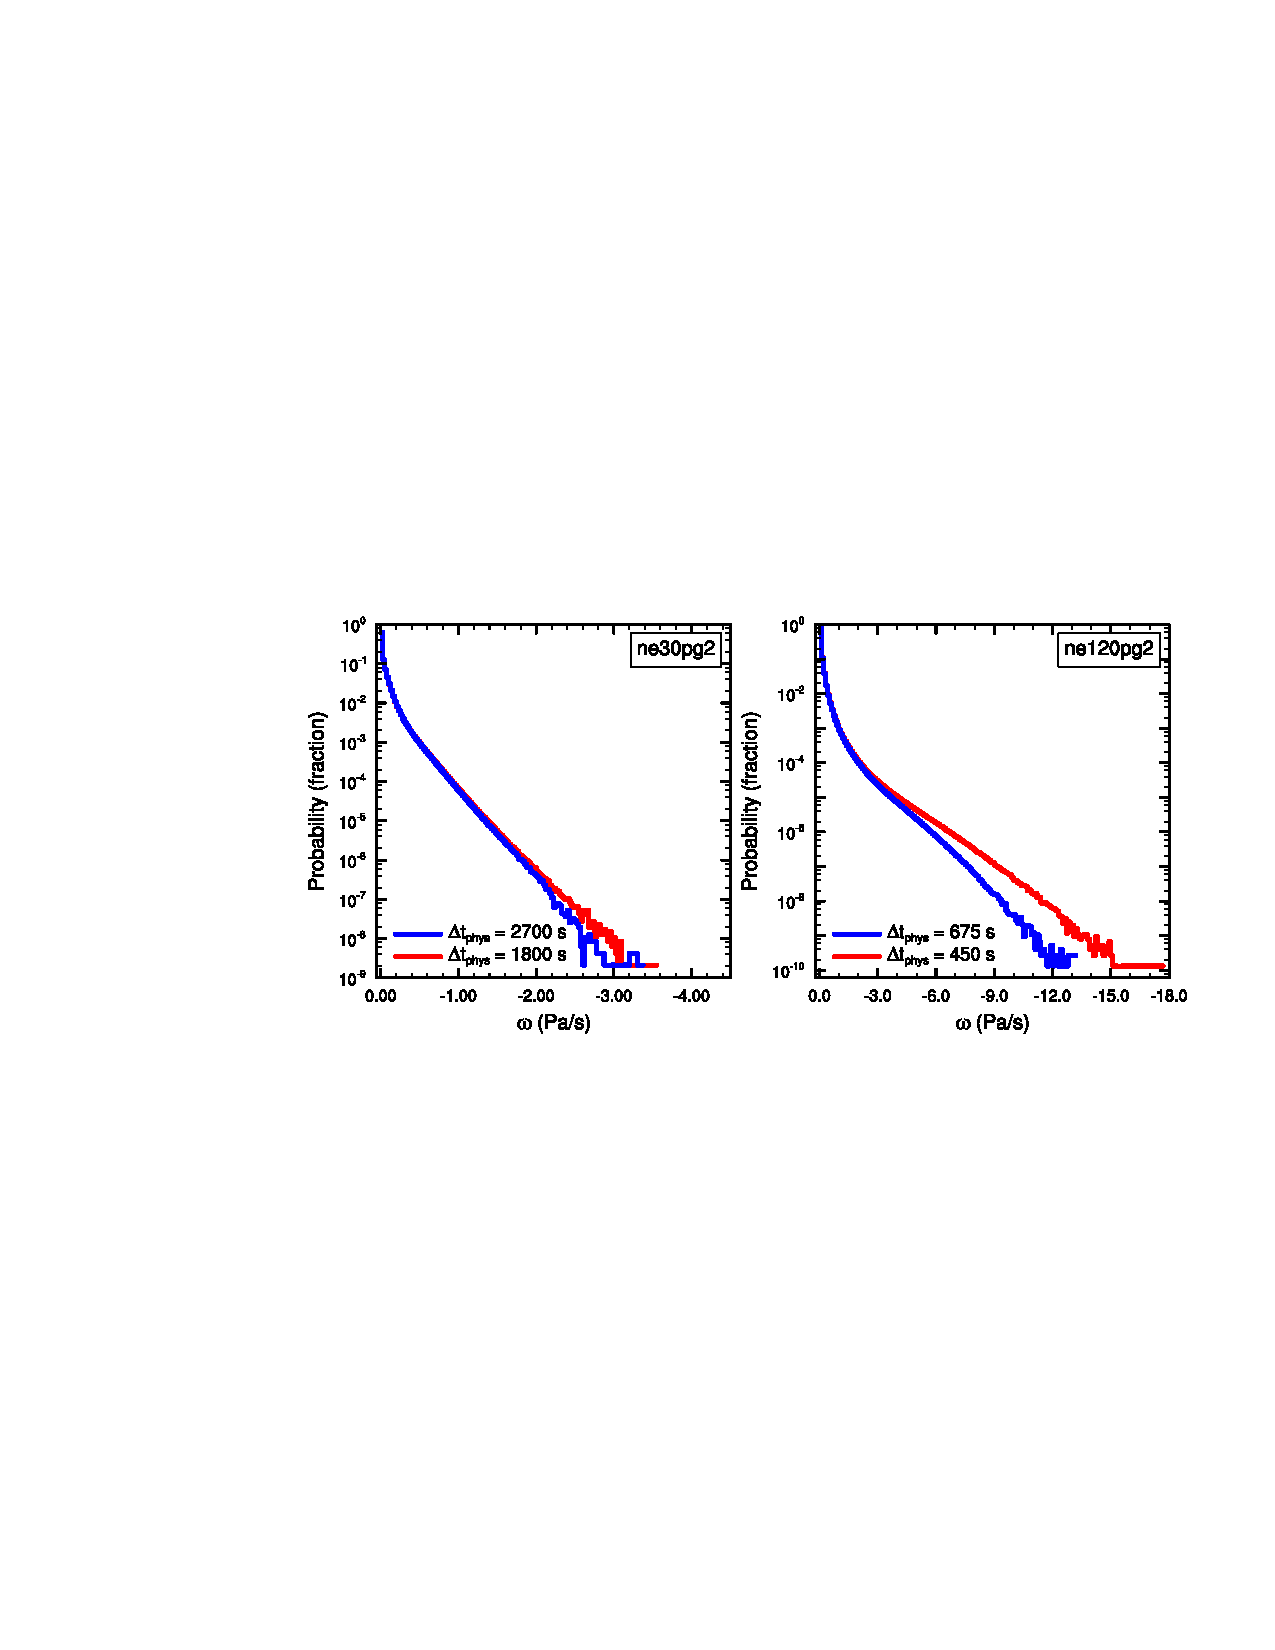
\includegraphics[width=20pc,angle=0]{chapter5/panel_pdf_dtphys.pdf}\\
\end{center}
\caption{Probability density distribution of upward $\omega$ everywhere in the model in the aqua-planets using the $ne30pg2$ grid (Left) and the $ne120pg2$ grid (Right). Figure computed for one year of 6-hourly data. The different colors indicate the physics time-steps used in the runs.}
\label{fig:pdf-dtphys}
\end{figure}

Figure~\ref{fig:pdf-dtphys} shows the PDFs of upward $\omega$ computed from a year of six-hourly data in the simulations. At lower resolution, $\Delta t_{phys}$ has only a very small effect on the solution, near the tale-end of the distributions. At high-resolution, values of $\omega$ less then about $-3 Pa/s$ are more frequent in the small $\Delta t_{phys}$ run, with the discrepancy growing more for larger magnitudes of $\omega$. The progressively larger errors with increasing resolution also manifests in the moist bubble tests, indicating that truncation errors arising from large $\Delta t_{phys}$ do exist in more complex configurations.

\subsection{The impact of high-order mapping to the dynamics grids}\label{sec:app2}

Figure~\ref{fig:loworder}a shows a close-up of the wavenumber power spectrum of the forcing on the $pg$ grid (dotted), where it is computed, and on the $GLL$ grid (solid), where it is has been mapped. In $ne30pg3$, the magnitudes are similar on both grids, except the mapping tends to damp the high wavenumbers of the forcing on the $GLL$ grid (greater than 60), but these scales are primarily below the effective resolution of the model and should not effect the solution. For $ne30pg2$, the magnitude of the forcing is actually greater after mapping to the $GLL$ grid, and more similar to the forcing in the $ne30pg3$ simulations. The high-order mapping can therefore replicate the scales of the physics tendencies that occur in the $pg3$ simulation, even though the physics are evaluated on a coarser $pg2$ grid.

\begin{figure}[t]
\begin{center}
\noindent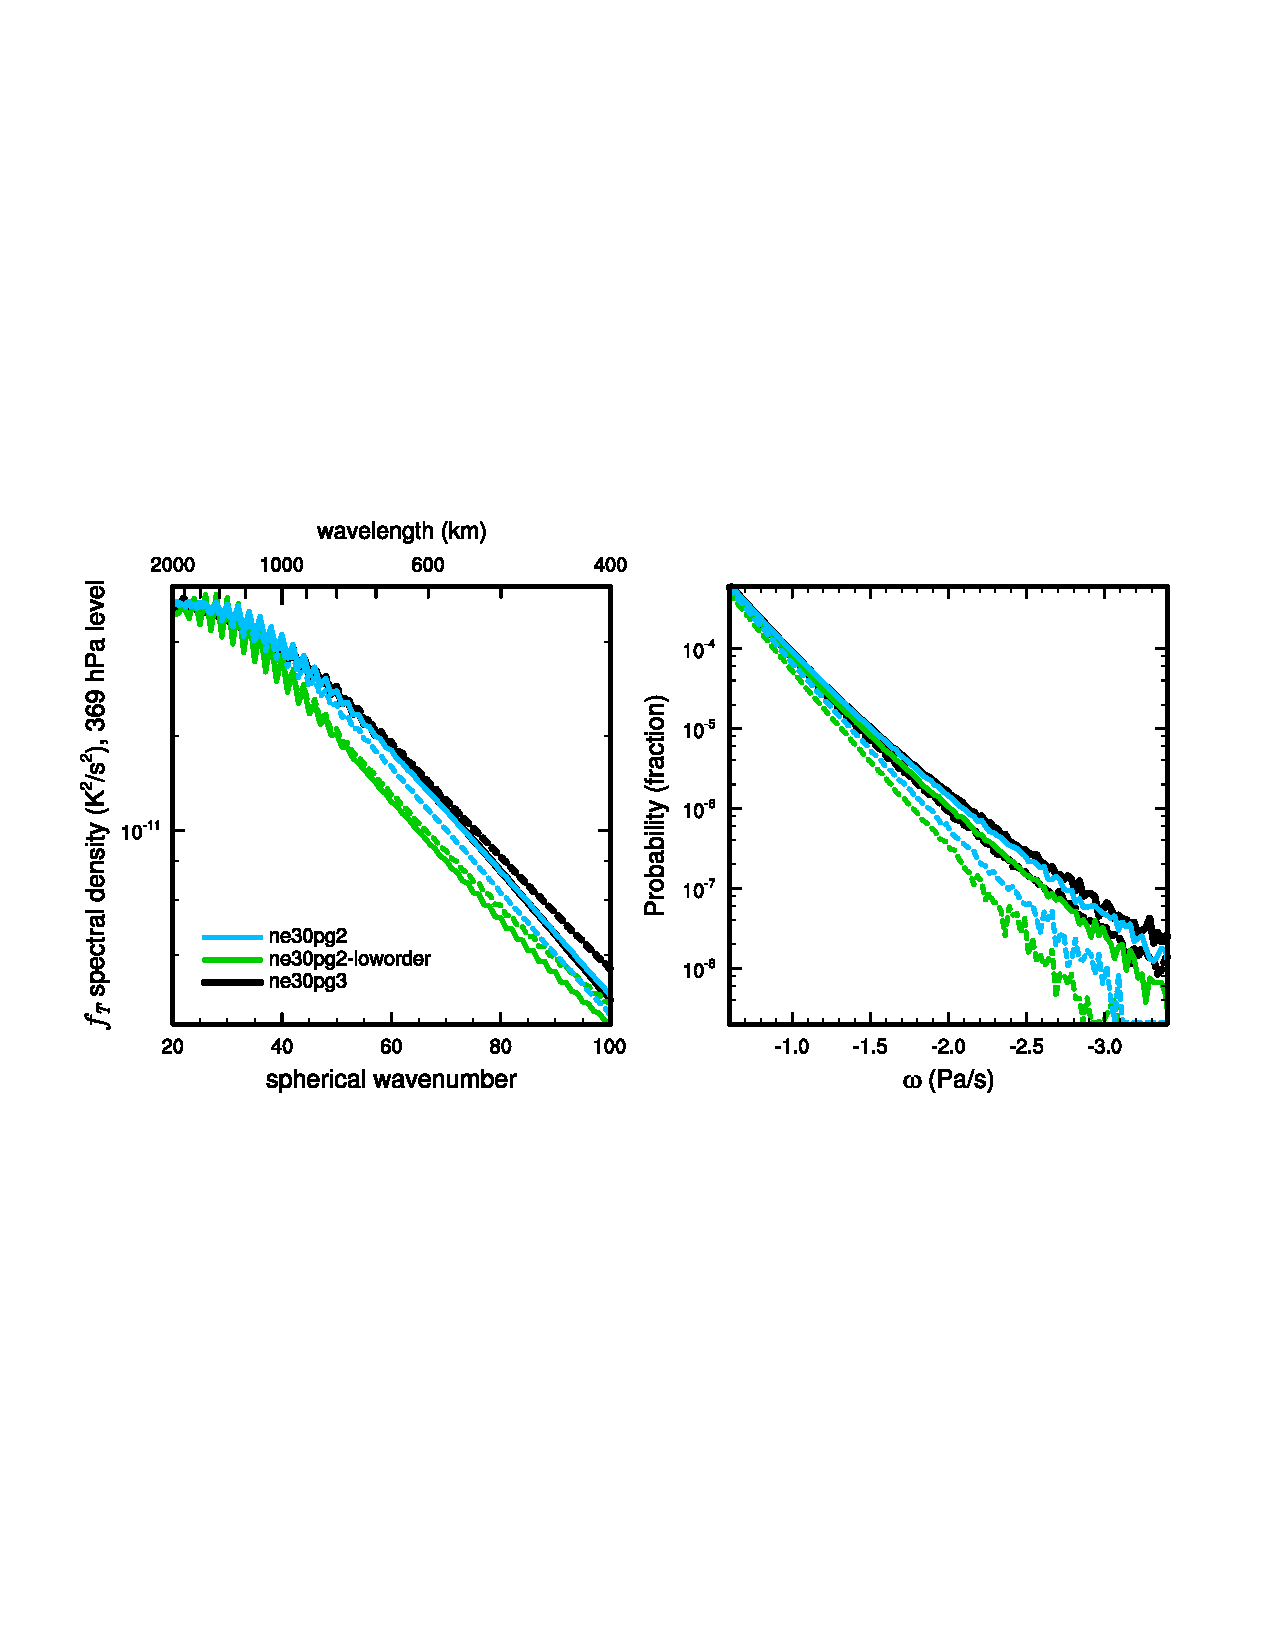
\includegraphics[width=30pc,angle=0]{chapter5/panel_loworder.pdf}\\
\end{center}
\caption{(Left) Wavenumber-power spectrum of the temperature tendencies from the moist physics, at the 369 hPa level, and (right) probability density distribution of upward $\omega$, everywhere in the model, for three year-long aqua-planet simulations. Solid lines refer to values of on the $GLL$ grids, and dashed lines, the fields on the $pg$ grids. See text for details regarding the three simulations.}
\label{fig:loworder}
\end{figure}

The importance of the high-order mapping can be shown with an additional $ne30pg2$ simulation, using low-order mapping ($ne30pg2-loworder$ in Figure~\ref{fig:loworder}). Specifically, low-order mapping refers to piecewise constant mapping between the $pg2$ and $CSLAM$ grids, and bi-linear mapping from $pg2$ to the $GLL$ grid. The forcing spectrum is now similar on both the $pg2$ and $GLL$ grids, although the low-order mapping tends to damp the forcing on the $GLL$ grid for wavenumbers greater than about 60, scales smaller than the models effective resolution (Figure~\ref{fig:loworder}a). A close up of the PDF of $\omega^{(gll)}$ is provided in Figure~\ref{fig:loworder}b (solid lines). As expected, the frequency of large magnitude $\omega^{(gll)}$ in the low-order run is less compared to the default $ne30pg2$ simulation. 

The dotted lines in Figure~\ref{fig:loworder}b show the PDF of $\omega$ on the $pg$ grids. The frequency of large magnitude $\omega$ is reduced on the $pg$ grids, compared to the state on the $GLL$ grids. This is primarily due to the smoothing effect of integrating the nodal point values over control volumes (H18). The larger $\omega$ values are even less frequent on the $pg2$ grid due to integrating over control volumes $\frac{9}{4}$ times greater than the $pg3$ control volumes. 

